\chapter{Technical Architecture, Implementation, and Deployment}

\section{Introduction}
This chapter covers the technical architecture of Riaya, the implementation choices of the Pengguin team, and the deployment strategy that put the product into production. It starts with an overview of the system architecture and the decision to split the project into two repositories, the web application and the voice server. It then goes through the technology stack component by component: frontend, backend, database, voice server, third-party integrations, background jobs, and CI/CD infrastructure. A section of screenshots shows the main features of the platform. The chapter ends with security, confidentiality, and access management, and with the technical challenges the team met and how it solved them.

\section{Global System Architecture}

\subsection{Architectural Principles}
Three architectural principles guided the technical decisions behind Riaya: \textit{separation of concerns}, \textit{event-driven communication}, and \textit{containerized deployment} \cite{fowler2002patterns}. They follow common cloud-native practice and keep the platform maintainable, scalable, and resilient as it grows.

Separation of concerns led to splitting Riaya into two independent repositories. Event-driven communication shows in the heavy use of WebSockets for real-time notifications between the web application and the voice server \cite{fette2011websocket}. Containerized deployment means every component runs in an isolated, reproducible environment managed by Docker \cite{docker2024}.

\subsection{Separation into Two Repositories (Web App and Voice Server)}
One of the team's first architectural decisions was to split Riaya into two repositories:

\begin{itemize}
    \item \textbf{Web App Repository:} Built with Next.js \cite{nextjs2024}, this repository contains the frontend and backend of the doctor and administrator dashboards. It manages authentication, patient records, appointments, invoices, medical documentation, subscriptions, and the WhatsApp configuration page. It communicates with the PostgreSQL database \cite{postgresql2024} through Drizzle ORM \cite{drizzle2024}.
    
    \item \textbf{Voice Server Repository:} Built with Express.js \cite{express2024}, this repository is dedicated to real-time communication. It handles incoming Twilio \cite{twilio2024} calls, WebSocket media streams, the OpenAI Realtime API \cite{openai2024realtime} integration (via Microsoft Azure \cite{azure2024openai}), WhatsApp integration using WhatsApp Baileys \cite{baileys2024}, and background jobs managed by BullMQ \cite{bullmq2024} and Redis \cite{redis2024}.
\end{itemize}

The split has four advantages. The two applications scale independently, which matters because the voice server streams real-time audio and needs very different resources from the web application. Failures stay isolated: a problem in the voice server does not take down the doctor dashboard, and the reverse is also true. The team can deploy one repository without redeploying the other, which speeds up delivery. And each application has a smaller attack surface and access to fewer sensitive credentials.

\begin{figure}[H]
    \centering
    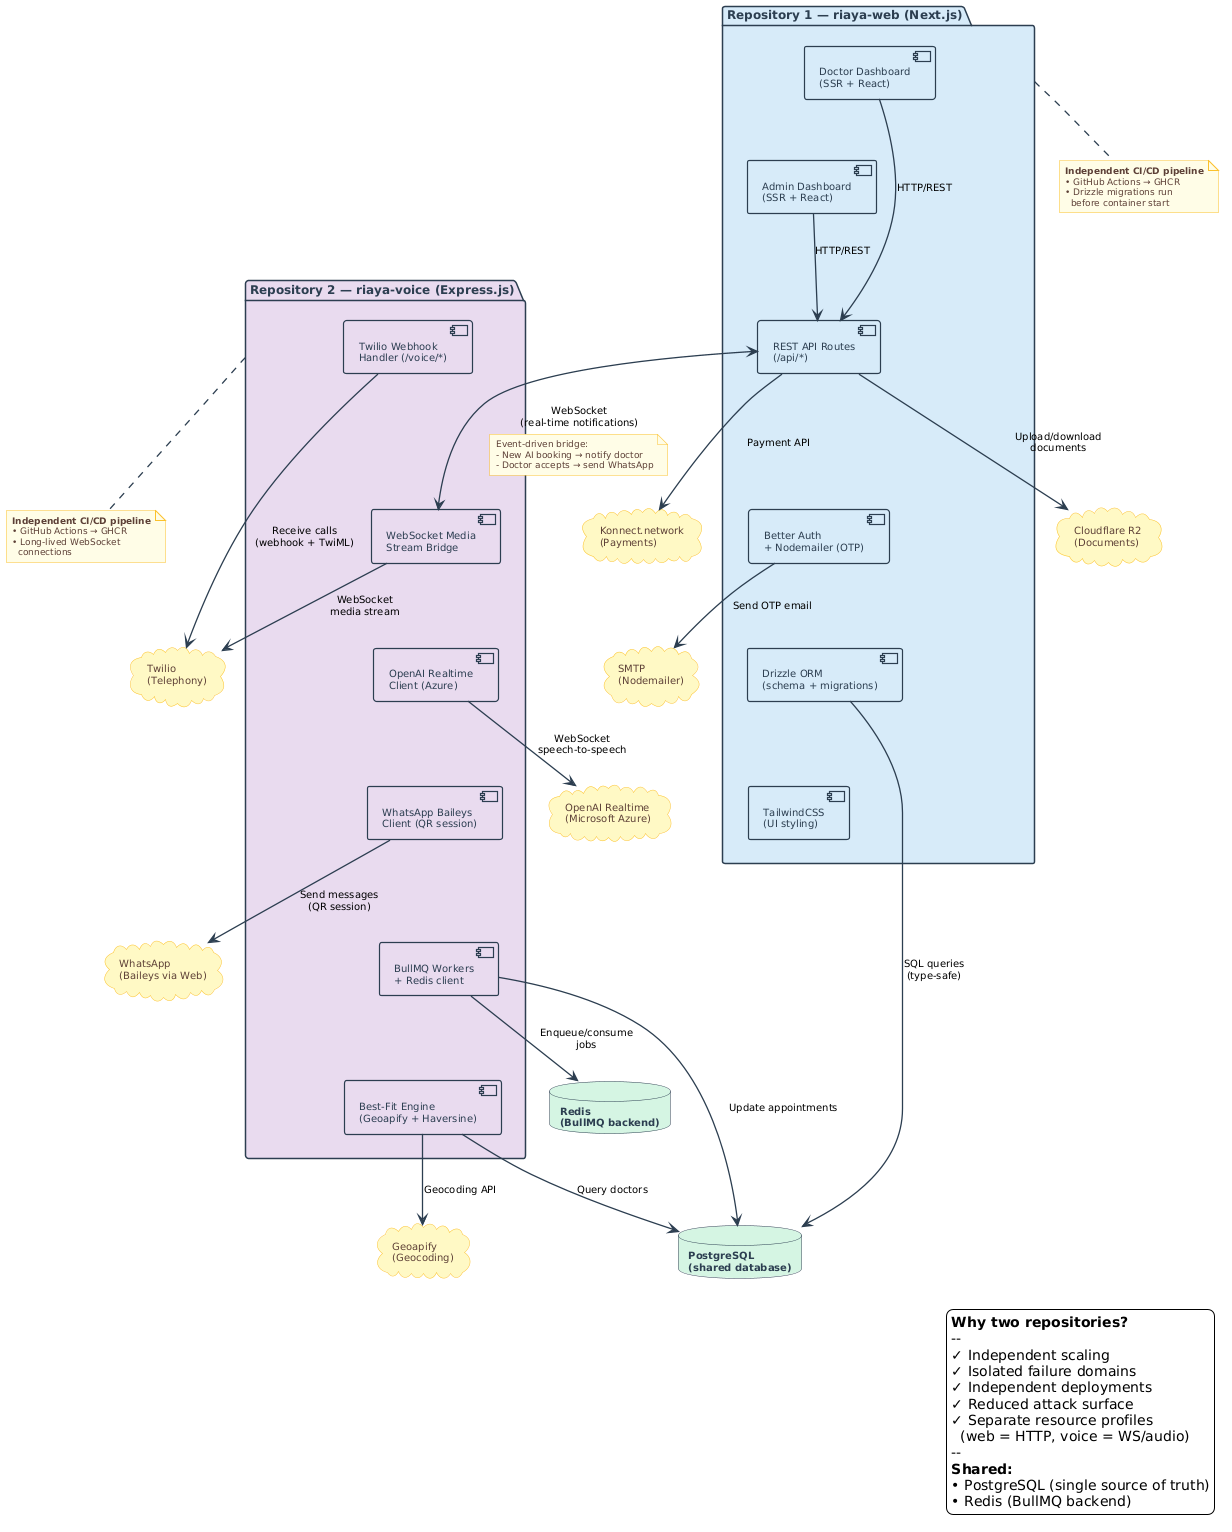
\includegraphics[width=0.85\textwidth,height=0.4\textheight,keepaspectratio]{images/two_repositories_architecture.png}
    \caption{Separation of the Riaya Platform into Two Repositories}
    \label{fig:two_repos}
\end{figure}

Figure~\ref{fig:two_repos} shows the two repositories, each with its own responsibilities and CI/CD pipeline.

\subsection{Technical Architecture Schema (Microservices, Event-Driven)}
Riaya is not a full microservices architecture \cite{newman2015microservices}, but it is service-oriented and event-driven. It is made of loosely coupled components that communicate through well-defined interfaces:

\begin{itemize}
    \item \textbf{Web Application:} Handles HTTP requests, renders the dashboard, and exposes REST endpoints for the doctor and administrator interfaces. It communicates with the database through Drizzle ORM.
    
    \item \textbf{Voice Server:} Handles Twilio webhooks, establishes WebSocket connections, and bridges the audio stream between Twilio and OpenAI Realtime API.
    
    \item \textbf{Database:} A PostgreSQL instance shared by both applications. It stores all persistent data, including doctor profiles, patients, appointments, invoices, consultations, subscriptions, and call logs.
    
    \item \textbf{Redis and BullMQ:} Used for background jobs and scheduled tasks, such as sending review requests two hours after an appointment, generating recurring invoices, and handling timeouts.
    
    \item \textbf{External Services:} Twilio (telephony), OpenAI Realtime API via Microsoft Azure (AI voice agent), Cloudflare R2 \cite{cloudflare2024r2} (file storage), Konnect.network \cite{konnect2024} (payments), WhatsApp Baileys (messaging), and Geoapify \cite{geoapify2024} (geocoding).
\end{itemize}

WebSockets carry the real-time notifications. When the voice server creates a new AI booking, it notifies the web application, which pushes the notification to the doctor's dashboard over a WebSocket. When a doctor accepts or declines an appointment, the web application notifies the voice server, which sends the patient a WhatsApp confirmation.

\begin{figure}[H]
    \centering
    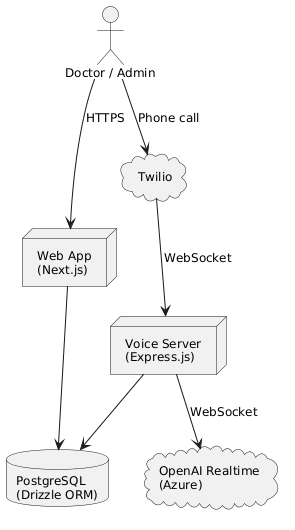
\includegraphics[width=0.85\textwidth,height=0.45\textheight,keepaspectratio]{images/global_architecture_schema.png}
    \caption{Global Technical Architecture of the Riaya Platform}
    \label{fig:global_arch}
\end{figure}

Figure~\ref{fig:global_arch} shows the global technical architecture of Riaya, with all components and their interactions.

\section{Technology Stack and Component Description}
This section goes through the technology stack of Riaya component by component and explains each choice in terms of performance, maintainability, and fit with the project requirements.

\subsection{Frontend and Backend Web: Next.js, TailwindCSS, Better Auth}
The web application is built with \textbf{Next.js} \cite{nextjs2024}, a React framework that supports server-side rendering (SSR), static site generation (SSG), and API routes. The team chose it for its performance, its built-in routing, and because a single codebase can hold both the frontend and the backend. The App Router was preferred over the Pages Router: nested layouts, streaming, and server actions made the complex dashboard pages simpler to build.

Styling uses \textbf{TailwindCSS} \cite{tailwind2024}, a utility-first CSS framework for building responsive interfaces quickly. The team chose it for its flexibility, its small bundle size after tree-shaking, and the consistent design system it enforces across the application.

\textbf{Better Auth} \cite{betterauth2024} handles authentication, with support for email and password, OTP, and session management. When a doctor registers, Riaya emails a one-time password (OTP) using \textbf{Nodemailer}. The OTP is stored in the Drizzle verification table, and the doctor must enter it to complete registration. This mechanism follows the NIST SP 800-63B recommendations on out-of-band authenticators \cite{nist2017sp80063b}.

\begin{figure}[H]
    \centering
    \begin{subfigure}[b]{0.22\textwidth}
        \centering
        
\includegraphics[width=\textwidth,height=2.2cm,keepaspectratio]{images/nextjs.png}
        \caption{Next.js}
        \label{fig:logo_nextjs}
    \end{subfigure}
    \hfill
    \begin{subfigure}[b]{0.22\textwidth}
        \centering
        
\includegraphics[width=\textwidth,height=2.2cm,keepaspectratio]{images/tailwindcss.png}
        \caption{TailwindCSS}
        \label{fig:logo_tailwind}
    \end{subfigure}
    \hfill
    \begin{subfigure}[b]{0.22\textwidth}
        \centering
        
\includegraphics[width=\textwidth,height=2.2cm,keepaspectratio]{images/better-auth.png}
        \caption{Better Auth}
        \label{fig:logo_betterauth}
    \end{subfigure}
    \hfill
    \begin{subfigure}[b]{0.22\textwidth}
        \centering
        
\includegraphics[width=\textwidth,height=2.2cm,keepaspectratio]{images/nodemailer.png}
        \caption{Nodemailer}
        \label{fig:logo_nodemailer}
    \end{subfigure}
    \caption{Logos of the frontend and backend web technologies}
    \label{fig:logos_frontend}
\end{figure}

Figure~\ref{fig:logos_frontend} shows the logos of the web stack technologies.

\subsection{Database: PostgreSQL and Drizzle ORM}
The main database is \textbf{PostgreSQL} \cite{postgresql2024}, an open-source relational database known for its reliability, scalability, and support for advanced data types. The team chose it for complex queries, ACID transactions, and its compatibility with Drizzle ORM. A relational database fits better than a NoSQL store here because the data (appointments, invoices, consultations) is highly structured and needs strong referential integrity.

\textbf{Drizzle ORM} \cite{drizzle2024} is a TypeScript-first ORM. Developers define schemas in TypeScript and Drizzle generates the SQL queries, with type checking that catches errors early and speeds up development. The team preferred it to Prisma because it generates lighter SQL and maps more directly to SQL semantics. Drizzle handles all database operations, including migrations, which run automatically during deployment before the new container starts.

\begin{figure}[H]
    \centering
    \begin{subfigure}[b]{0.3\textwidth}
        \centering
        
\includegraphics[width=\textwidth,height=2.5cm,keepaspectratio]{images/postgresql.png}
        \caption{PostgreSQL}
        \label{fig:logo_postgres}
    \end{subfigure}
    \caption{Logo of the PostgreSQL database}
    \label{fig:logo_postgres_main}
\end{figure}

\begin{figure}[H]
    \centering
    
\includegraphics[width=0.85\textwidth,height=0.4\textheight,keepaspectratio]{images/postgresql_drizzle.png}
    \caption{PostgreSQL and Drizzle ORM Stack}
    \label{fig:postgres_drizzle}
\end{figure}

Figure~\ref{fig:postgres_drizzle} shows how PostgreSQL and Drizzle ORM fit together in Riaya.

\subsection{Voice Server and Real-Time: Express.js, Twilio, OpenAI Realtime API (Microsoft Azure)}
The voice server is built with \textbf{Express.js} \cite{express2024}, a minimalist Node.js framework for web applications and APIs, chosen for its simplicity, its performance, and its compatibility with WebSocket libraries such as \texttt{ws}.

\textbf{Twilio} \cite{twilio2024} receives the patients' phone calls. When a patient dials the Riaya number, Twilio sends a webhook to the Express.js server, which answers with TwiML (Twilio Markup Language) that opens a WebSocket media stream from Twilio to the server. Through this stream, the server receives live audio from the patient's phone and sends audio back.

The AI voice agent runs on the \textbf{OpenAI Realtime API} \cite{openai2024realtime}, accessed through \textbf{Microsoft Azure} \cite{azure2024openai}. Its speech-to-speech mode lets the AI understand the patient and answer in real time. The agent speaks English, French, and Tunisian Arabic, and it calls tools in the Riaya system to search for doctors, check availability, and create appointments. Azure was chosen as the host because its regional deployments reduce network latency for users in North Africa.

\begin{figure}[H]
    \centering
    \begin{subfigure}[b]{0.22\textwidth}
        \centering
        
\includegraphics[width=\textwidth,height=2.2cm,keepaspectratio]{images/expressjs.png}
        \caption{Express.js}
        \label{fig:logo_express}
    \end{subfigure}
    \hfill
    \begin{subfigure}[b]{0.22\textwidth}
        \centering
        
\includegraphics[width=\textwidth,height=2.2cm,keepaspectratio]{images/twilio.png}
        \caption{Twilio}
        \label{fig:logo_twilio}
    \end{subfigure}
    \hfill
    \begin{subfigure}[b]{0.22\textwidth}
        \centering
        
\includegraphics[width=\textwidth,height=2.2cm,keepaspectratio]{images/openai.png}
        \caption{OpenAI}
        \label{fig:logo_openai}
    \end{subfigure}
    \hfill
    \begin{subfigure}[b]{0.22\textwidth}
        \centering
        
\includegraphics[width=\textwidth,height=2.2cm,keepaspectratio]{images/azure.png}
        \caption{Microsoft Azure}
        \label{fig:logo_azure}
    \end{subfigure}
    \caption{Logos of the voice server and real-time communication technologies}
    \label{fig:logos_voice}
\end{figure}

\begin{figure}[H]
    \centering
    
\includegraphics[width=0.85\textwidth,height=0.4\textheight,keepaspectratio]{images/voice_server_stack.png}
    \caption{Voice Server and Real-Time Stack}
    \label{fig:voice_stack}
\end{figure}

Figures~\ref{fig:logos_voice} and~\ref{fig:voice_stack} present the voice server stack.

\subsection{Third-Party Integrations: WhatsApp Baileys, Cloudflare R2, Konnect.network}
\textbf{WhatsApp Baileys} \cite{baileys2024} is a library that connects to WhatsApp Web and sends messages from code. Doctors link their own WhatsApp number by scanning a QR code, so every message goes out from the doctor's own number and the conversation between doctor and patient stays private.

\textbf{Cloudflare R2} \cite{cloudflare2024r2} stores uploaded medical documents and files. It is S3-compatible object storage with low latency, high durability, and no egress fees.

\textbf{Konnect.network} \cite{konnect2024} processes the Pro plan payments, including the recurring invoices generated by a daily BullMQ job.

\begin{figure}[H]
    \centering
    \begin{subfigure}[b]{0.3\textwidth}
        \centering
        
\includegraphics[width=\textwidth,height=2.5cm,keepaspectratio]{images/whatsapp.png}
        \caption{WhatsApp Baileys}
        \label{fig:logo_whatsapp}
    \end{subfigure}
    \hfill
    \begin{subfigure}[b]{0.3\textwidth}
        \centering
        
\includegraphics[width=\textwidth,height=2.5cm,keepaspectratio]{images/cloudflare.png}
        \caption{Cloudflare R2}
        \label{fig:logo_cloudflare}
    \end{subfigure}
    \hfill
    \begin{subfigure}[b]{0.3\textwidth}
        \centering
        
\includegraphics[width=\textwidth,height=2.5cm,keepaspectratio]{images/konnect.png}
        \caption{Konnect.network}
        \label{fig:logo_konnect}
    \end{subfigure}
    \caption{Logos of the third-party integrations}
    \label{fig:logos_thirdparty}
\end{figure}

Figure~\ref{fig:logos_thirdparty} shows the logos of the third-party integrations.

\subsection{Background Jobs and Cache: BullMQ, Redis}
\textbf{BullMQ} \cite{bullmq2024} is a Node.js library for background jobs and scheduled tasks. It runs on \textbf{Redis} \cite{redis2024}, an in-memory data store used for caching and message brokering. In Riaya, BullMQ handles several critical tasks:
\begin{itemize}
    \item Sending a WhatsApp review message two hours after a confirmed appointment ends.
    \item Generating recurring invoices for Pro subscriptions that are about to expire.
    \item Handling timeouts for pending appointments (auto-cancellation after 10 minutes).
    \item Sending callbacks or WhatsApp notifications to patients when a pending request expires.
\end{itemize}

The team chose BullMQ over simpler options such as node-cron for its reliability, retry policies, and observability. Its dashboard shows job status in real time.

\begin{figure}[H]
    \centering
    \begin{subfigure}[b]{0.3\textwidth}
        \centering
        
\includegraphics[width=\textwidth,height=2.5cm,keepaspectratio]{images/bullmq.png}
        \caption{BullMQ}
        \label{fig:logo_bullmq}
    \end{subfigure}
    \hfill
    \begin{subfigure}[b]{0.3\textwidth}
        \centering
        
\includegraphics[width=\textwidth,height=2.5cm,keepaspectratio]{images/redis.png}
        \caption{Redis}
        \label{fig:logo_redis}
    \end{subfigure}
    \caption{Logos of the background jobs and cache technologies}
    \label{fig:logos_background}
\end{figure}

\begin{figure}[H]
    \centering
    
\includegraphics[width=0.8\textwidth,height=0.4\textheight,keepaspectratio]{images/bullmq_redis.png}
    \caption{Background Jobs and Cache Stack (BullMQ and Redis)}
    \label{fig:bullmq_redis}
\end{figure}

Figures~\ref{fig:logos_background} and~\ref{fig:bullmq_redis} present the background jobs and cache stack.

\subsection{Infrastructure and CI/CD: Docker, GitHub Actions, Ubuntu VPS, Nginx}
Riaya runs in \textbf{Docker} \cite{docker2024} containers managed by \textbf{Docker Compose} on a self-hosted \textbf{Ubuntu VPS}. Each repository has its own \textbf{GitHub Actions} CI/CD workflow: on every push to the \texttt{main} branch, GitHub-hosted runners build the Docker images, publish them to the \textbf{GitHub Container Registry (GHCR)}, and deploy the updated containers to the VPS.

On the VPS, \textbf{Nginx} acts as a reverse proxy in front of the application containers and handles TLS termination and routing. PostgreSQL and Redis run as containers on a shared Docker network, which the web and voice containers join. Web deployments run the Drizzle migrations before the new container starts. This setup follows the continuous delivery principles of Humble and Farley \cite{humble2010continuous}.

\begin{figure}[H]
    \centering
    \begin{subfigure}[b]{0.22\textwidth}
        \centering
        
\includegraphics[width=\textwidth,height=2.2cm,keepaspectratio]{images/docker.png}
        \caption{Docker}
        \label{fig:logo_docker}
    \end{subfigure}
    \hfill
    \begin{subfigure}[b]{0.22\textwidth}
        \centering
        
\includegraphics[width=\textwidth,height=2.2cm,keepaspectratio]{images/github-actions.png}
        \caption{GitHub Actions}
        \label{fig:logo_ghactions}
    \end{subfigure}
    \hfill
    \begin{subfigure}[b]{0.22\textwidth}
        \centering
        
\includegraphics[width=\textwidth,height=2.2cm,keepaspectratio]{images/ubuntu.png}
        \caption{Ubuntu}
        \label{fig:logo_ubuntu}
    \end{subfigure}
    \hfill
    \begin{subfigure}[b]{0.22\textwidth}
        \centering
        
\includegraphics[width=\textwidth,height=2.2cm,keepaspectratio]{images/nginx.png}
        \caption{Nginx}
        \label{fig:logo_nginx}
    \end{subfigure}
    \caption{Logos of the infrastructure and CI/CD technologies}
    \label{fig:logos_infra}
\end{figure}

Figure~\ref{fig:logos_infra} presents the logos of the infrastructure and CI/CD technologies.

\section{Screenshots and Detailed Descriptions}
This section shows the main screens of Riaya, grouped by interface, with a description of what each one does. Together they show how the functional requirements of Chapter~1 were implemented.

\subsection{Admin Interface: Dashboard and Statistics}
The admin home page gives an overview of the whole platform. It shows key statistics, such as the number of registered doctors, appointments, and AI calls, along with charts of platform trends, doctor activity, and usage.

\IfFileExists{images/admin_dashboard_home.png}{%
\begin{figure}[H]
    \centering
    \includegraphics[width=0.85\textwidth,height=0.5\textheight,keepaspectratio]{images/admin_dashboard_home.png}
    \caption{Admin Dashboard Home Page}
    \label{fig:admin_home}
\end{figure}
}{}

\subsection{Doctor Interface: Appointment Calendar and Urgent Badges}
Doctors see and manage their schedule in a calendar view. New AI requests appear in real time over WebSockets. Urgent requests carry a badge and trigger a stronger live notification for the doctor, which the urgent booking flow described in Section~\ref{subsec:urgencies} depends on.

\begin{figure}[H]
    \centering
    
\includegraphics[width=0.85\textwidth,height=0.5\textheight,keepaspectratio]{images/doctor_calendar.png}
    \caption{Doctor Appointment Calendar with Urgent Badges}
    \label{fig:doctor_calendar}
\end{figure}

Figure~\ref{fig:doctor_calendar} shows the doctor's appointment calendar with urgent badges.

\subsection{Doctor Interface: WhatsApp Configuration and QR Code Generation}
On this page, doctors link their personal WhatsApp number by scanning a QR code. Once connected, every message goes out from the doctor's own number, which keeps conversations private. The page also shows the connection status and lets the doctor disconnect the session.

\begin{figure}[H]
    \centering
    
\includegraphics[width=0.85\textwidth,height=0.5\textheight,keepaspectratio]{images/doctor_whatsapp_config.png}
    \caption{WhatsApp Configuration Page with QR Code}
    \label{fig:doctor_whatsapp}
\end{figure}

Figure~\ref{fig:doctor_whatsapp} shows the WhatsApp configuration page with QR code generation.

\subsection{Doctor Interface: Invoice Management and WhatsApp Sending}
Doctors create, edit, and cancel invoices on this page, and send an invoice to the patient on WhatsApp with one click. The page also shows the payment status (paid or unpaid) and the invoice history.

\begin{figure}[H]
    \centering
    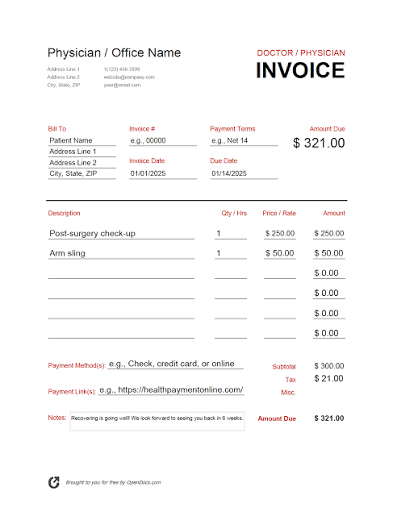
\includegraphics[width=0.85\textwidth,height=0.5\textheight,keepaspectratio]{images/doctor_invoice.png}
    \caption{Invoice Management Page}
    \label{fig:doctor_invoice}
\end{figure}

Figure~\ref{fig:doctor_invoice} shows the invoice management page.

\subsection{Admin Interface: Live Call Monitoring and Transcriptions}
On this page, administrators follow ongoing calls between the AI agent and patients in real time. It shows the live transcript, the patient's name, and the call status, which the team relies on for operations and debugging.

\begin{figure}[H]
    \centering
    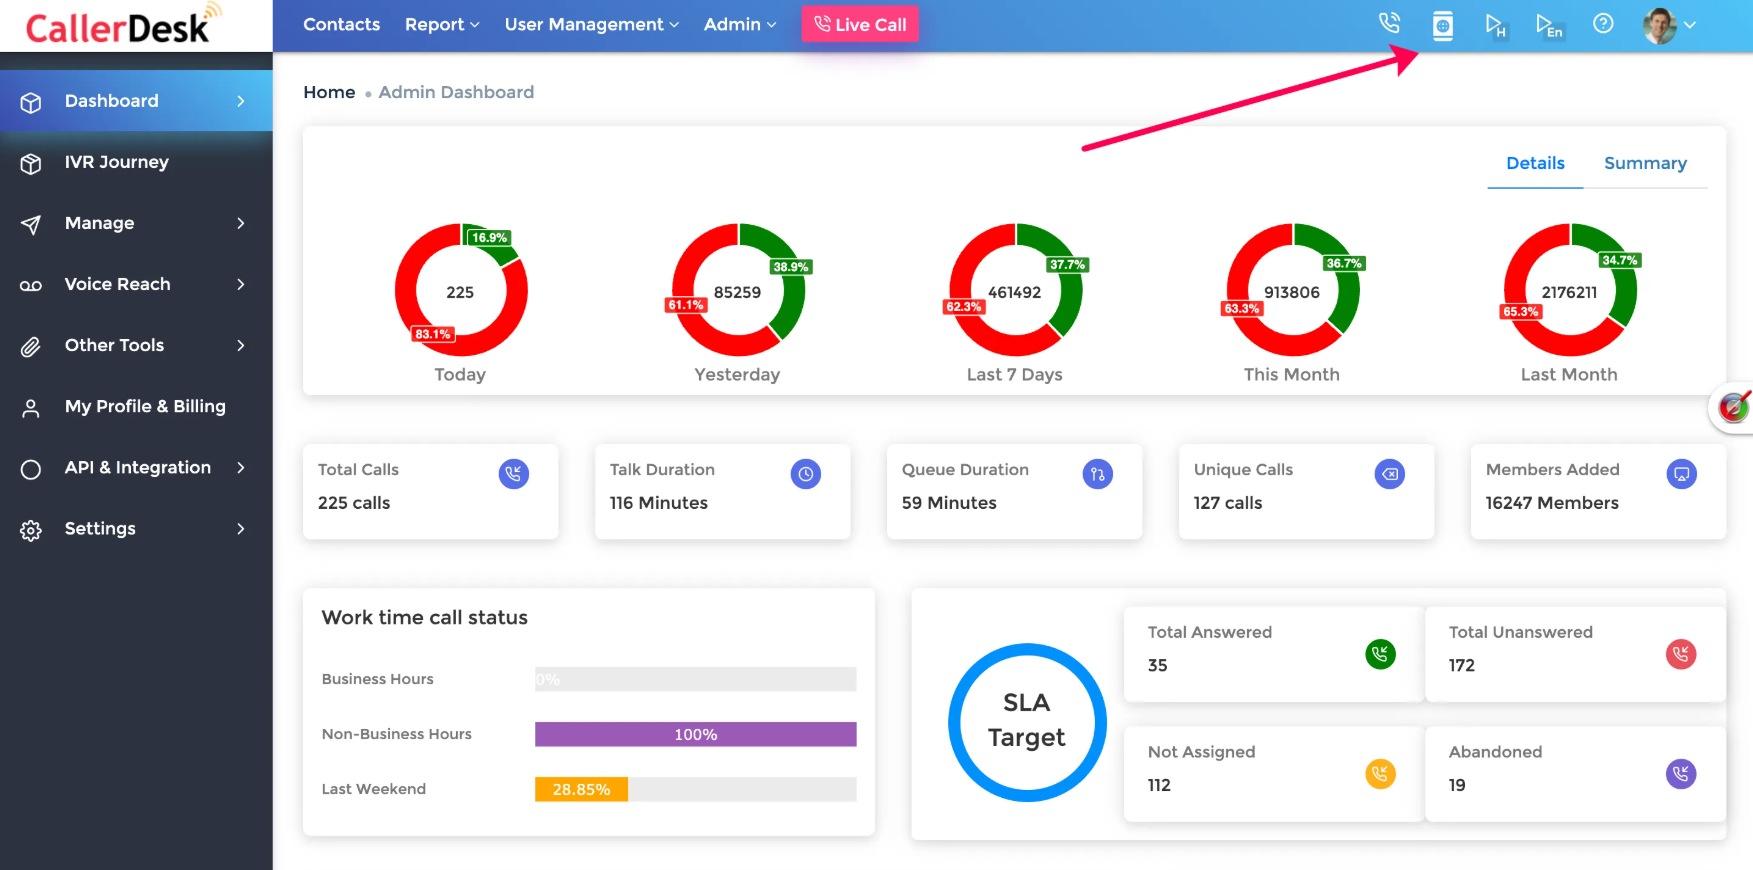
\includegraphics[width=0.85\textwidth,height=0.5\textheight,keepaspectratio]{images/admin_live_call.png}
    \caption{Admin Live Call Monitoring Interface}
    \label{fig:admin_live_call}
\end{figure}

Figure~\ref{fig:admin_live_call} shows the admin live call monitoring interface.

\subsection{Admin Interface: Doctor Verification and Best-Fit Search}
On the doctor verification page, administrators browse and search doctor applications and approve or reject them, optionally with reasons shown to the doctor. The best-fit search page runs the same search algorithm the AI uses, so administrators can check on a map and a calendar which doctors match a speciality, location, and date range.

\begin{figure}[H]
    \centering
    
\includegraphics[width=0.85\textwidth,height=0.5\textheight,keepaspectratio]{images/admin_doctor_verification.png}
    \caption{Admin Doctor Verification Interface}
    \label{fig:admin_verification}
\end{figure}

\begin{figure}[H]
    \centering
    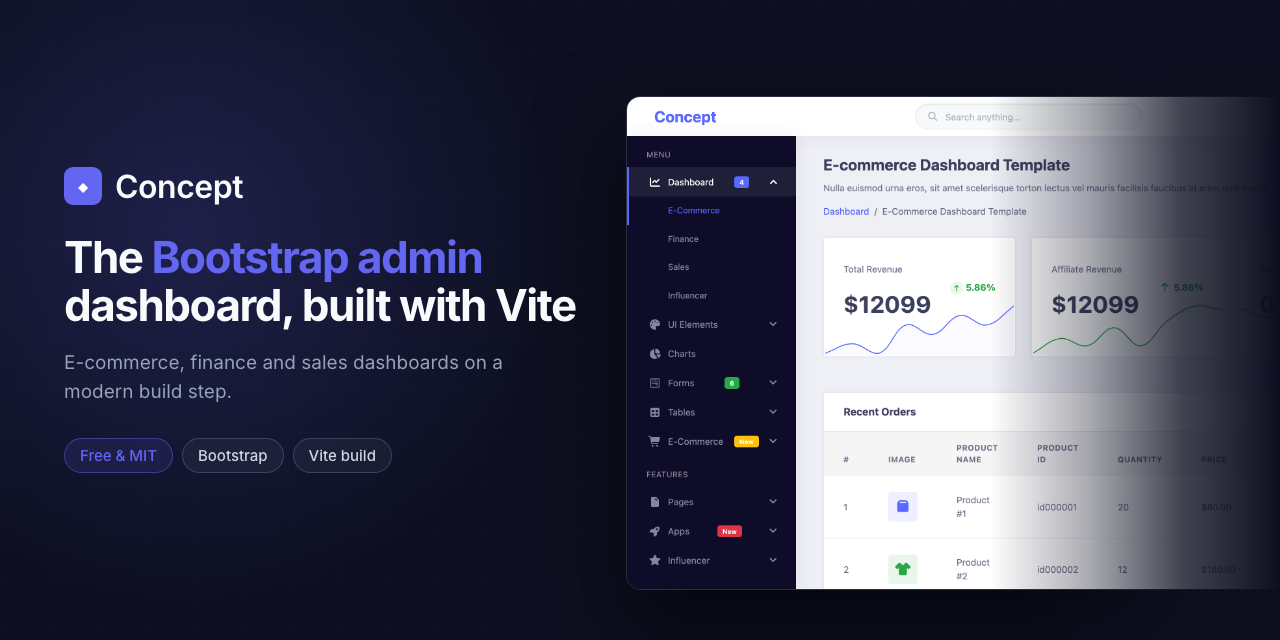
\includegraphics[width=0.85\textwidth,height=0.5\textheight,keepaspectratio]{images/admin_bestfit_search.png}
    \caption{Admin Best-Fit Search Interface}
    \label{fig:admin_bestfit}
\end{figure}

Figures~\ref{fig:admin_verification} and~\ref{fig:admin_bestfit} show the doctor verification and best-fit search interfaces.

\subsection{Database: ERD Diagram and Drizzle Migrations}
The ERD shows the database schema, and the terminal output shows the Drizzle migration files running during deployment.

\begin{figure}[H]
    \centering
    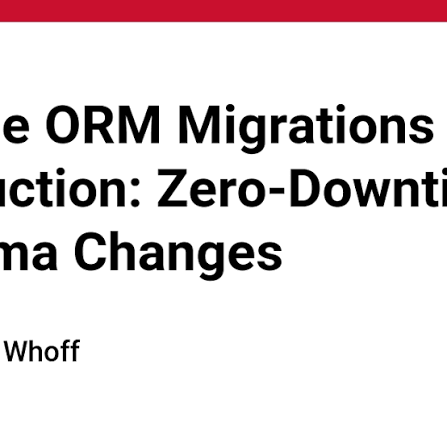
\includegraphics[width=0.85\textwidth,height=0.5\textheight,keepaspectratio]{images/erd_diagram_ch3.png}
    \caption{Entity-Relationship Diagram of the Riaya Database}
    \label{fig:erd_ch3}
\end{figure}

\begin{figure}[H]
    \centering
    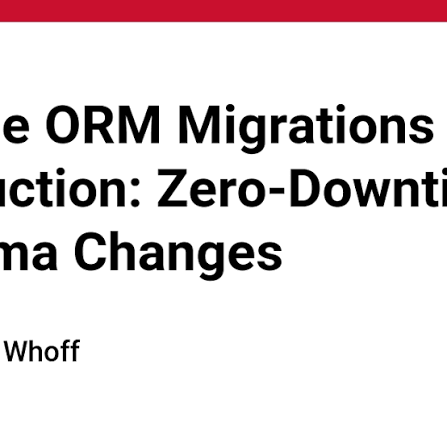
\includegraphics[width=0.85\textwidth,height=0.5\textheight,keepaspectratio]{images/drizzle_migrations.png}
    \caption{Drizzle Migrations Execution}
    \label{fig:drizzle_migrations}
\end{figure}

Figures~\ref{fig:erd_ch3} and~\ref{fig:drizzle_migrations} show the ERD and the Drizzle migrations.

\subsection{Twilio Console: Call Logs and Webhooks}
The Twilio console lists incoming calls and the webhooks that point to the Express.js voice server.

\begin{figure}[H]
    \centering
    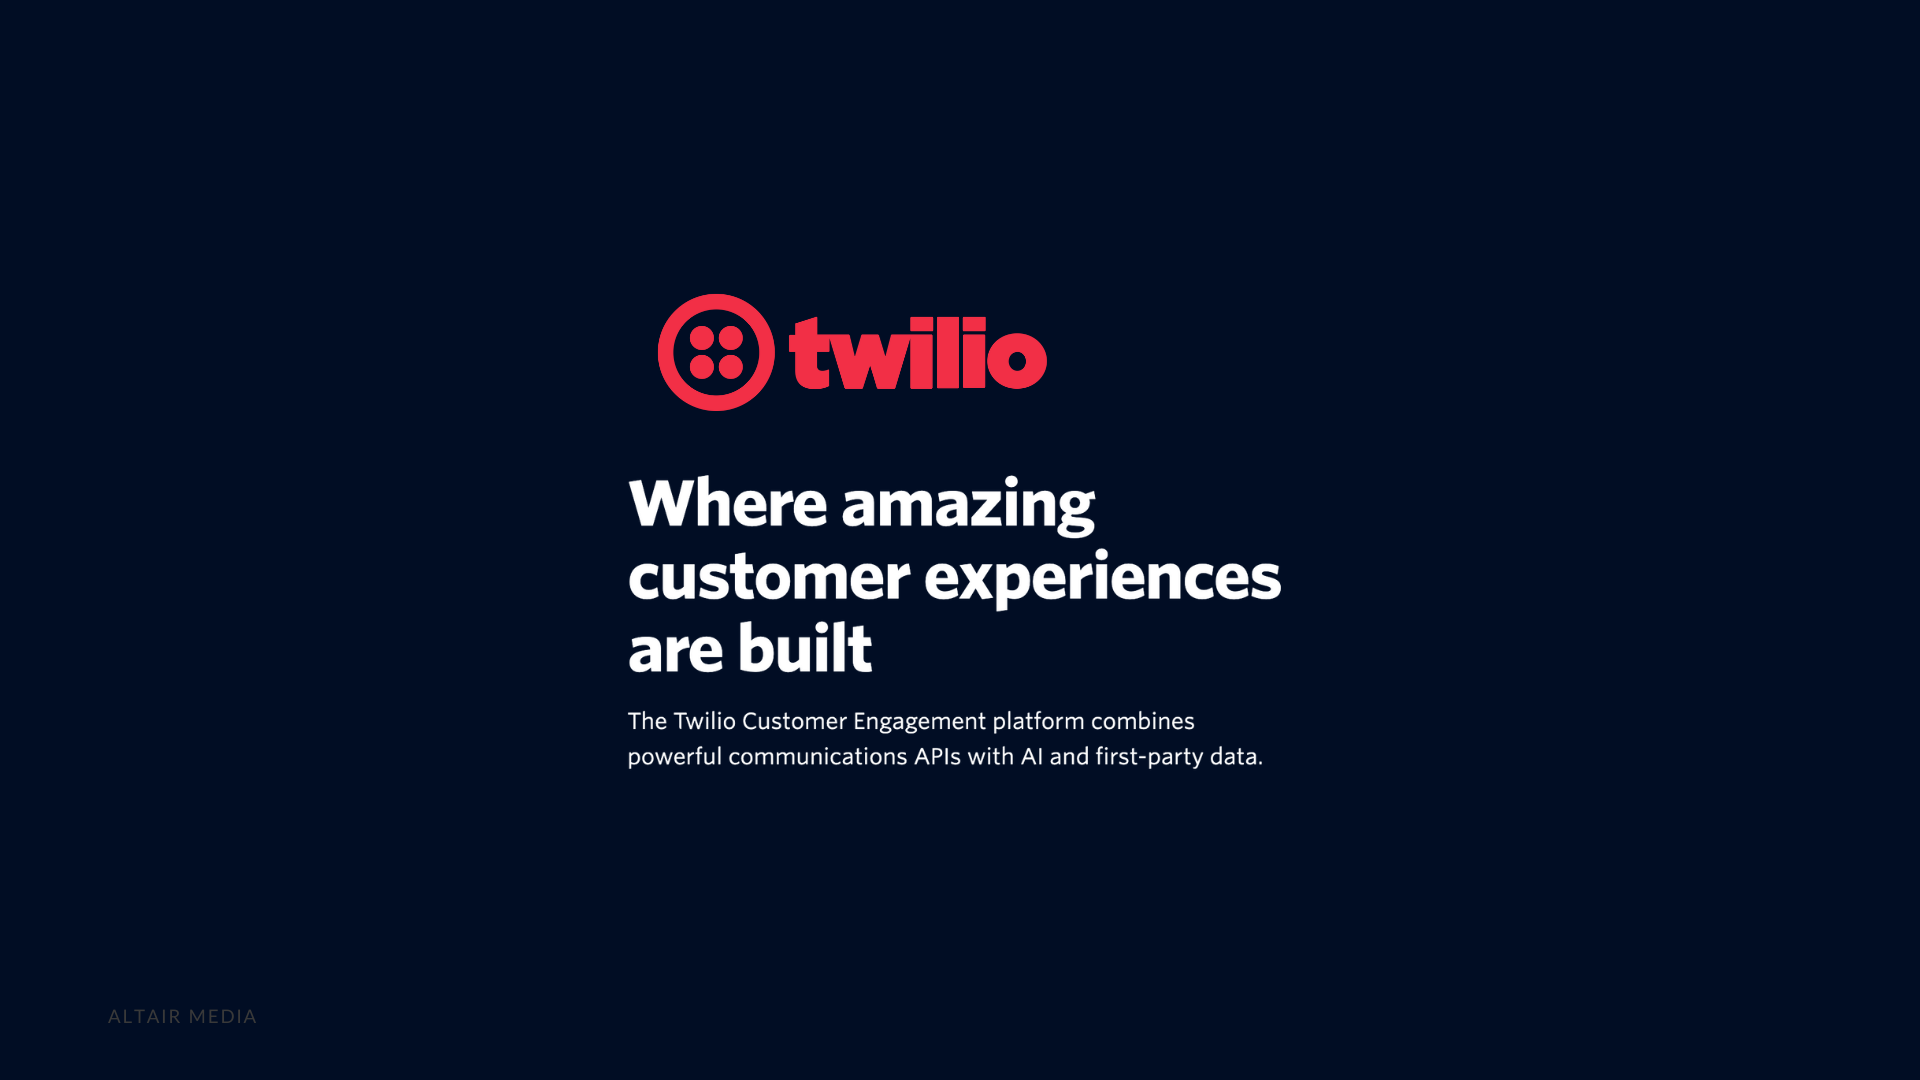
\includegraphics[width=0.85\textwidth,height=0.5\textheight,keepaspectratio]{images/twilio_console.png}
    \caption{Twilio Console with Call Logs and Webhooks}
    \label{fig:twilio_console}
\end{figure}

Figure~\ref{fig:twilio_console} shows the Twilio console with call logs and webhooks.

\subsection{Azure / OpenAI Portal: Voice Agent Configuration}
The Azure portal shows the deployment of the OpenAI Realtime model behind the AI voice agent and its configuration, including the language settings and the tool definitions.

\begin{figure}[H]
    \centering
    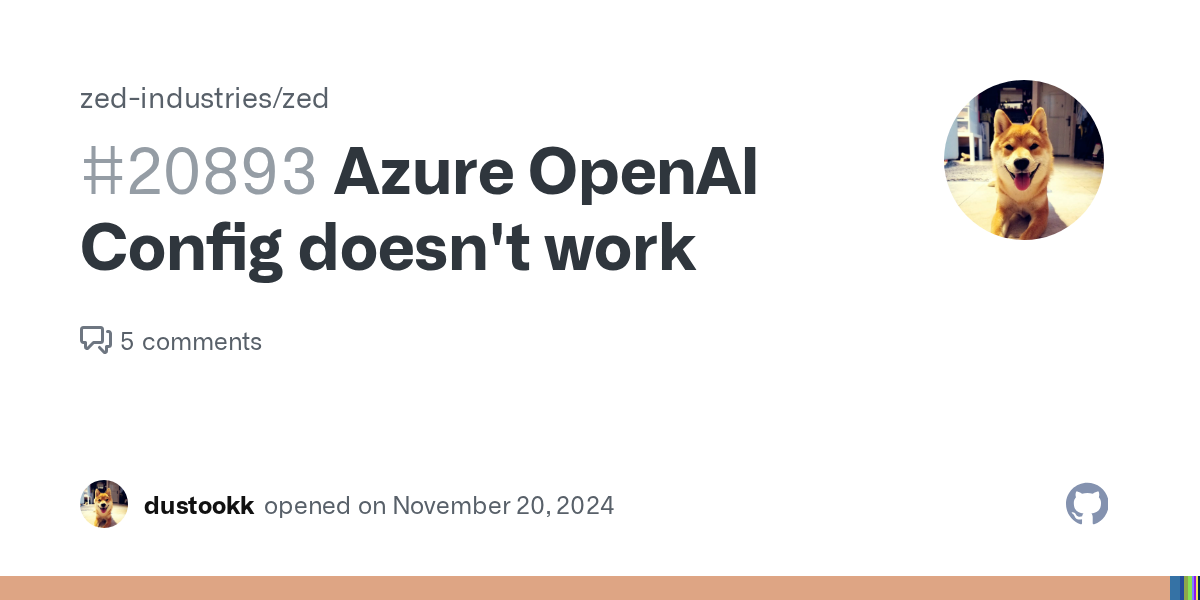
\includegraphics[width=0.85\textwidth,height=0.5\textheight,keepaspectratio]{images/azure_openai_config.png}
    \caption{Azure / OpenAI Portal Configuration}
    \label{fig:azure_openai}
\end{figure}

Figure~\ref{fig:azure_openai} shows the Azure / OpenAI portal configuration.

\subsection{BullMQ Dashboard (Redis Insight): Scheduled Jobs Monitoring}
The BullMQ dashboard, opened through Redis Insight, lists the scheduled jobs and their status (waiting, active, completed, failed). The team uses it to monitor background tasks such as review requests and recurring invoices.

\begin{figure}[H]
    \centering
    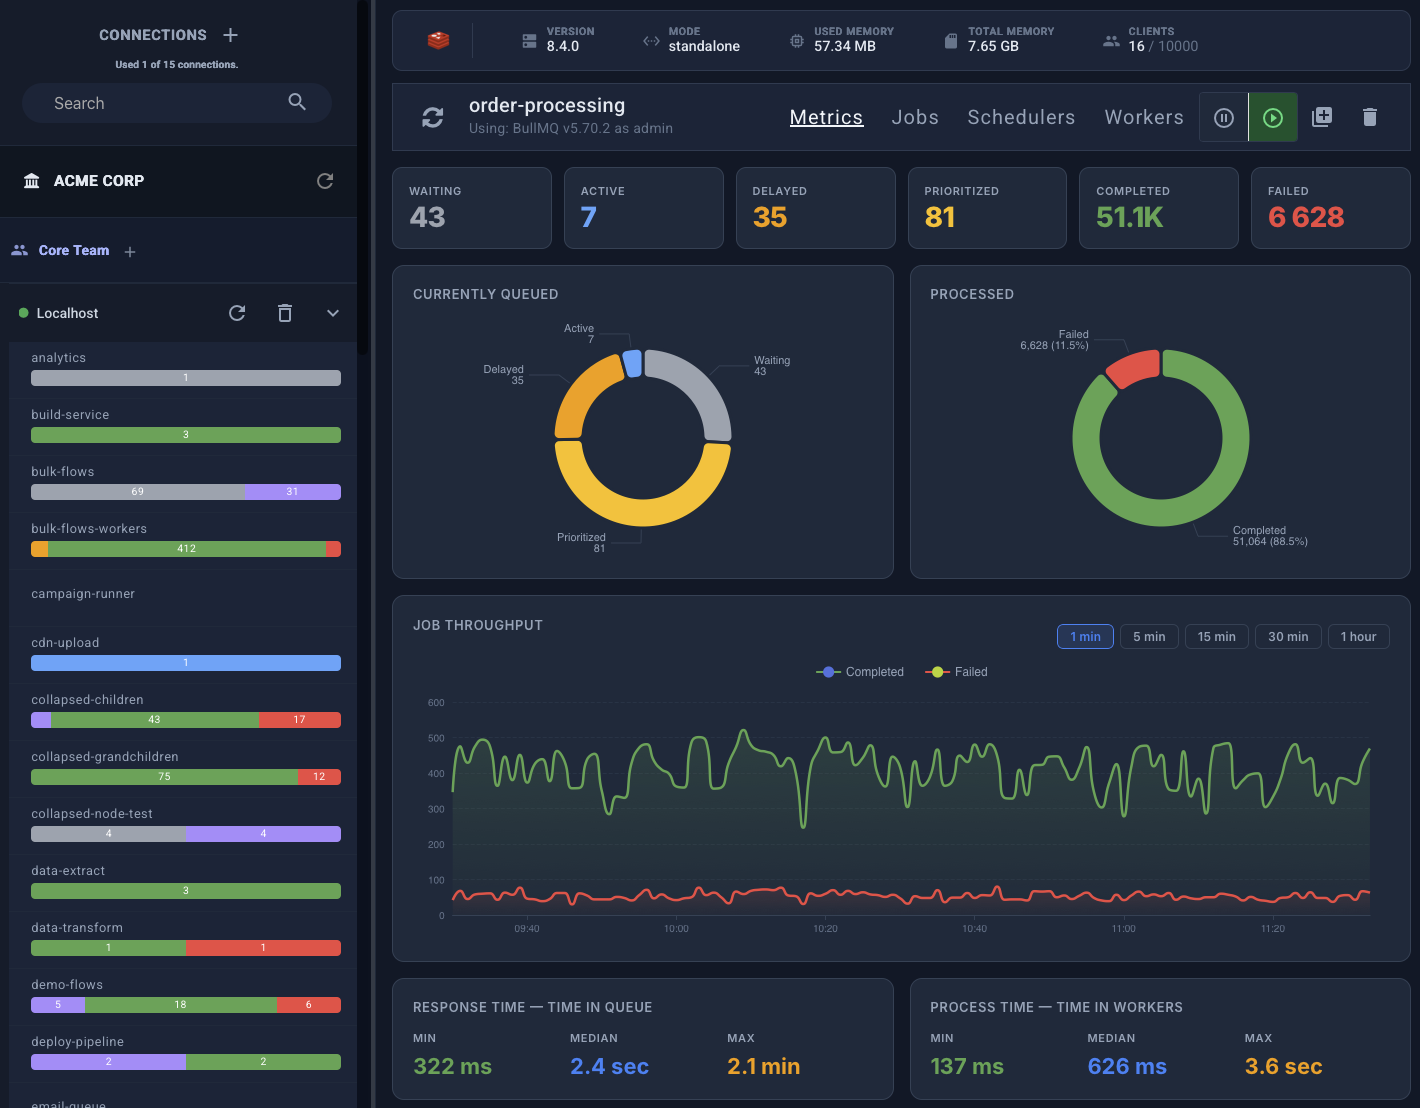
\includegraphics[width=0.85\textwidth,height=0.5\textheight,keepaspectratio]{images/bullmq_dashboard.png}
    \caption{BullMQ Dashboard for Scheduled Jobs}
    \label{fig:bullmq_dashboard}
\end{figure}

Figure~\ref{fig:bullmq_dashboard} shows the BullMQ dashboard for scheduled jobs.

\subsection{WhatsApp Baileys Logs: Connection and Message Sending}
The WhatsApp Baileys logs show the connection status of the doctor's WhatsApp session and each message as it is sent.

\begin{figure}[H]
    \centering
    
\includegraphics[width=0.85\textwidth,height=0.5\textheight,keepaspectratio]{images/whatsapp_baileys_logs.png}
    \caption{WhatsApp Baileys Connection and Message Logs}
    \label{fig:whatsapp_logs}
\end{figure}

Figure~\ref{fig:whatsapp_logs} shows the WhatsApp Baileys connection and message logs.

\subsection{GitHub Actions: CI/CD Workflow}
The GitHub Actions workflow shows each step of the automated CI/CD pipeline: building the Docker image, publishing it to GHCR, and deploying it to the VPS.

\begin{figure}[H]
    \centering
    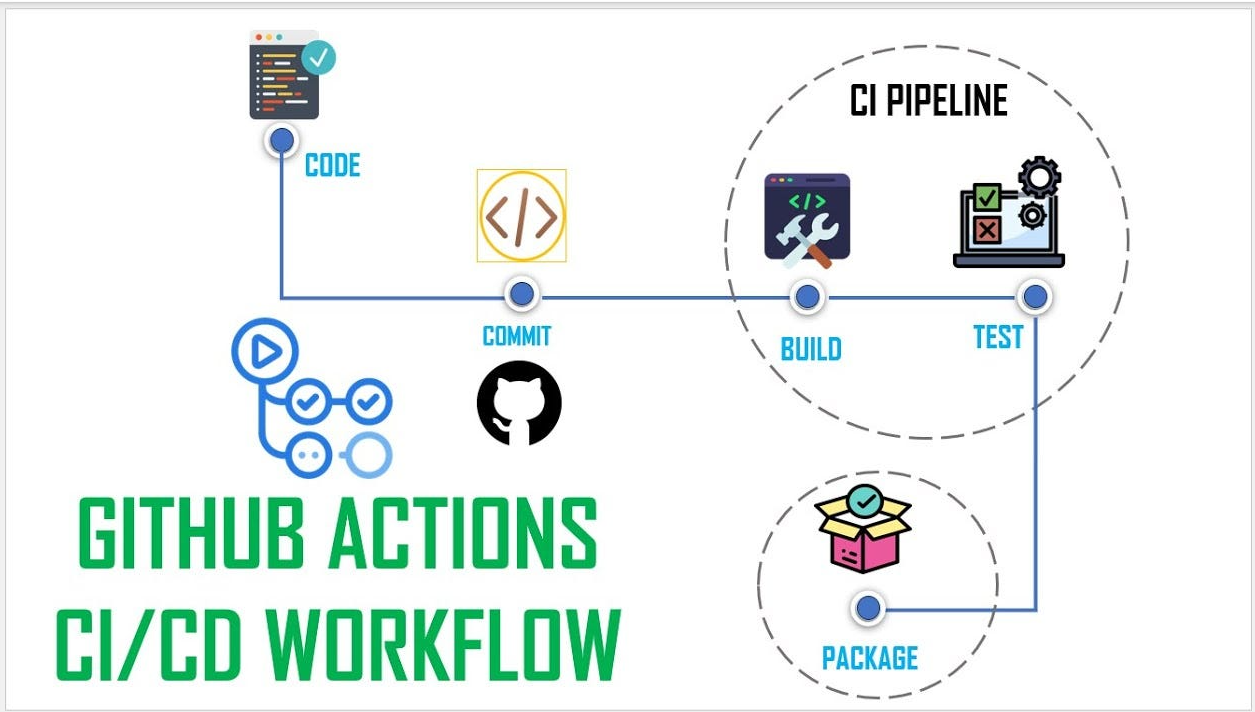
\includegraphics[width=0.85\textwidth,height=0.5\textheight,keepaspectratio]{images/github_actions_workflow.png}
    \caption{GitHub Actions CI/CD Workflow}
    \label{fig:github_actions}
\end{figure}

Figure~\ref{fig:github_actions} shows the GitHub Actions CI/CD workflow.

\subsection{Docker Compose: Running Containers on the VPS}
The Docker Compose output lists the containers running on the VPS (the web app, the voice server, PostgreSQL, Redis, and Nginx) and their health.

\begin{figure}[H]
    \centering
    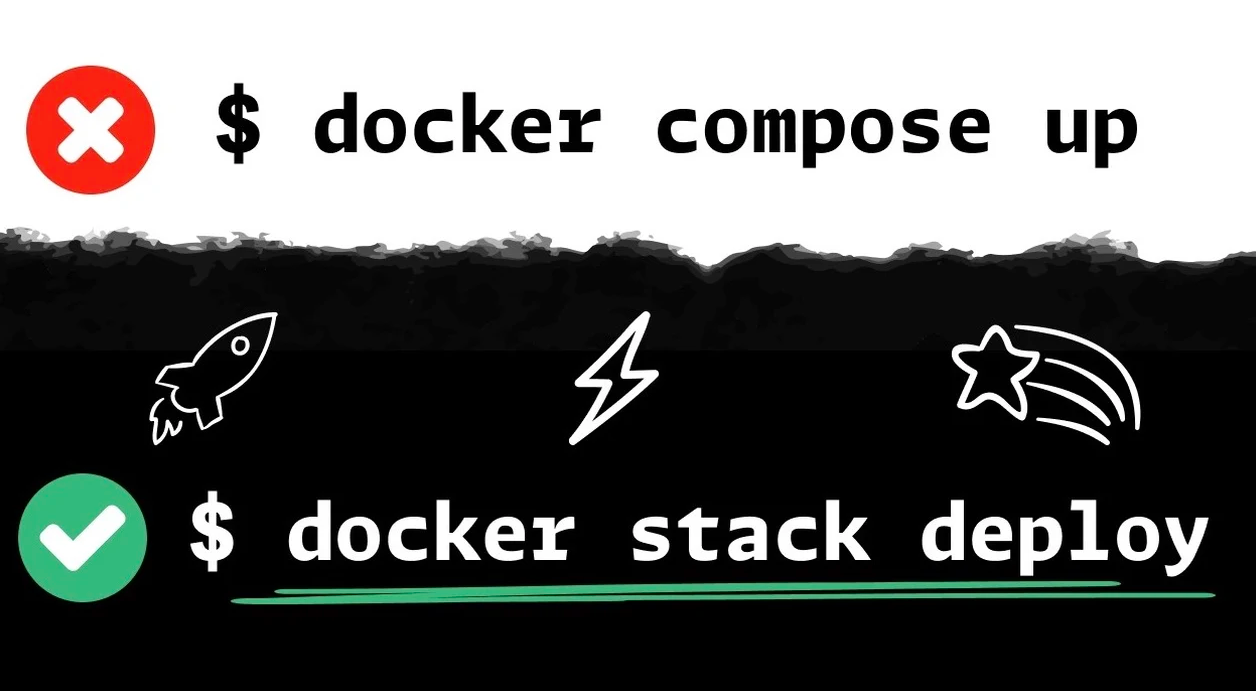
\includegraphics[width=0.85\textwidth,height=0.5\textheight,keepaspectratio]{images/docker_compose_vps.png}
    \caption{Docker Compose Running Containers on the VPS}
    \label{fig:docker_compose}
\end{figure}

Figure~\ref{fig:docker_compose} shows the Docker Compose output with running containers on the VPS.

\section{Security, Confidentiality, and Access Management}

\subsection{Authentication and Authorization (OTP, Better Auth, Roles)}
Better Auth handles authentication, with support for email and password, OTP, and session management. Doctors must verify their email with an OTP sent by Nodemailer before they can complete registration, and until an administrator approves the application, they can only reach the profile page. Authorization is role-based: doctors, administrators, and patients (who have no account) each have a different level of access. This follows the principle of least privilege recommended by OWASP \cite{owasp2024}.

\begin{table}[H]
    \centering
    \caption{Authentication and Authorization Matrix}
    \label{tab:auth_matrix}
    \small
    \begin{tabular}{p{2.5cm}p{3.5cm}p{3.5cm}p{3.5cm}}
        \toprule
        \textbf{Role} & \textbf{Authentication} & \textbf{Access Level} & \textbf{Restrictions} \\
        \midrule
        Patient & None (phone number) & Phone call + WhatsApp & No web access \\
        Doctor & Email OTP (Better Auth) & Full dashboard after approval & Profile only until approved \\
        Administrator & Email and password & Full back-office access & None \\
        \bottomrule
    \end{tabular}
\end{table}

Table~\ref{tab:auth_matrix} summarizes how each role authenticates and what it can access.

\subsection{Protection of Medical Data (Cloudflare R2, Compliance)}
Medical documents are stored in Cloudflare R2, which encrypts them at rest and in transit. Access is restricted to the doctor who uploaded a document and, where applicable, to the patient through WhatsApp. The platform must comply with Tunisian data protection regulations (INPDP) \cite{inpdp2004} and, where applicable, with the GDPR principles \cite{gdpr2016} of data minimization, purpose limitation, and the right to erasure. The team chose Cloudflare R2 for its S3-compatible API, its strong encryption, and its zero egress fees, which keep down the cost of storing large medical files.

\subsection{Confidentiality of WhatsApp Conversations}
WhatsApp messages go out through the doctor's own phone number (via WhatsApp Baileys), so the conversation between doctor and patient stays private, and Riaya has no access to the content of these messages once they are sent. The team chose this design to protect patient privacy and meet medical confidentiality requirements. It also spares the platform the data retention obligations it would have if it stored the messages itself.

\section{Technical Challenges Encountered and Solutions Adopted}

\subsection{Real-Time Latency Management (WebSockets, OpenAI Realtime)}
Latency was one of the main technical challenges. The voice server must relay audio between Twilio and the OpenAI Realtime API with minimal delay, or the conversation stops feeling natural. The team used WebSockets for low-latency communication, tuned the audio buffering strategy, and relied on Microsoft Azure's regional deployments to cut network latency. The target was under 500 ms end to end, the threshold usually given for natural conversation \cite{itu2003g114}.

\subsection{Best-Fit Algorithm (Haversine, Geoapify, Scoring)}
The best-fit algorithm was another hard problem. It has to resolve the patient's location, rank doctors by distance and availability, and return the top 2--3 options quickly. The team used Geoapify \cite{geoapify2024} for geocoding, the Haversine formula \cite{haversine1971} for distances, and a scoring function that combines distance and time difference. The algorithm is optimized to run within a few hundred milliseconds, so the patient is not kept waiting.

The scoring function is:
\[
\text{Score} = \text{distance (km)} + \frac{|\text{slot} - \text{preferred time}| \text{ (minutes)}}{10}
\]

\paragraph{Geocoding and Tunisian Locations.}
To find the patient's location, the platform uses Geoapify, which had the richest data among the services tested. It still has gaps: some addresses exist in several places, which makes them ambiguous. To compensate, the AI also receives a curated list of Tunisian cities and places, which helps it interpret what callers say and makes the best-fit search more accurate.

\subsection{Management of Urgencies and Timeouts}\label{subsec:urgencies}
The urgent booking flow and the timeout handling needed careful design. When the AI detects an urgent situation, it creates up to three pending appointments linked by an emergency group ID. The first doctor to accept gets the appointment, and the other requests are cancelled automatically. If no doctor accepts within 10 minutes, the whole group is cancelled and the patient is notified by a callback or a WhatsApp message. BullMQ schedules these tasks, and Redis holds their state. The mechanism draws on patterns from \textit{Enterprise Integration Patterns} \cite{hohpe2003eip}.

\subsection{Rejection Handling Workflow}
\label{subsec:rejection-handling}

One of the trickiest parts of the patient experience was deciding what happens when a doctor refuses an appointment or takes too long to answer. The team first considered asking the patient to choose a backup doctor up front, in case the first one refuses, but that would add yet another question to an already long call. The team chose a simpler approach: the patient picks one doctor, and if that doctor refuses, the platform calls the patient back with another option. This keeps the call as easy as possible for the patient. The team plans to test the approach further and may revise it if a better alternative appears.

\subsection{Pricing Display Decision}
\label{subsec:pricing-display}

Price matters when choosing a doctor, and the team first wanted to show prices on the platform. If only the first consultation price mattered, this would be easy. But the real cost depends on many factors, and two doctors with the same first consultation price can charge very different amounts for their services. The team considered letting doctors enter a price for each service, which works for services with a fixed price, such as braces. In most cases, though, patients do not know what they need before a diagnosis, and an AI cannot reliably handle a diagnosis over the phone. The team therefore decided not to show full prices, so patients are not misled and the platform stays focused on booking rather than medical pricing.

\subsection{Voice Model Evaluation and Selection}
\label{subsec:voice-model-evaluation}

The phone call is the most important feature of Riaya, so the team put a lot of effort into choosing the AI models and the architecture behind it. This section covers the two main ways to build an AI phone call, the testing method, the problem of Tunisian Arabic, the approaches tested, the results, and the final choice.

\subsubsection{Two Approaches to Build a Phone Call}
There are two fundamentally different ways to build an AI-powered phone call. The first is \emph{speech-to-speech} (realtime): a single model listens to the caller and answers with its own voice. This approach is fast and feels natural. The second is a \emph{chain of steps}: the caller's voice is converted to text (STT), an AI model generates the answer (LLM), and the answer is converted back to voice (TTS). This gives more control because the best model can be chosen for each step, but every step adds waiting time. The team tested both approaches.

\subsubsection{Testing Methodology}
The team built a small program that acts like a phone caller. It plays the same seven sentences each time, covering Tunisian Arabic, French, and mixed sentences such as \textit{``\foreignlanguage{arabic}{نحب ناخذ} rendez-vous \foreignlanguage{arabic}{عند} dermatologue''}. The program records the AI's answers and measures the response time. The real application instructions and booking tools were used, so the AI behaved as it would in production. Each step was also timed individually to identify bottlenecks. To compare fairly, a test call page was built where the engine could be switched and the same call run on each one. One limitation: the test voices were computer-generated, not real patients.

\subsubsection{The Challenge of Tunisian Arabic}
For English and French, almost every speech-to-text and voice model tested performed well. Tunisian Arabic (Derja) was where the models differed significantly, and it was the main problem from the start. Few models understand it: one model returned nothing for Arabic, while others dropped or misspelled words. Mixed sentences with French words inside Arabic were the hardest. Few voices speak it well: Gemini had the most natural Arabic voices, while Inworld offered only two Arabic voices that were not perfect. Every choice was judged on Tunisian Arabic first, because that is how the patients speak.

\subsubsection{Approach 1: Realtime Models (Speech-to-Speech)}
The team started with Azure OpenAI Realtime and then tested Gemini Live for comparison. GPT Realtime had a very good response time and followed instructions well, but its pronunciation was not perfect. Gemini Live also had a very good response time and the best voice, but it could not follow instructions carefully and lost track of the conversation. The ``extended thinking'' version often failed to use the results of the booking tools (8 out of 18 tries in the test). On response time, both were fast: Gemini Live answered in 1.6 to 4.5 seconds, faster when answering immediately and slower when calling a tool first.

\subsubsection{Approach 2: Chain of Steps with Inworld.ai}
Next, the team tried the chain of steps, first with Inworld.ai. The AI models available there were not great, and it answered in about 2.2 seconds in the test call. Inworld also has only two Arabic voices, which were not perfect.

\subsubsection{Approach 3: LiveKit Agents with Different Models}
After that, LiveKit agents were used. They allow choosing the model for every step, so many combinations could be tested. The comparison table below comes from these tests. Inworld was mainly used as a speech-to-text and text-to-speech provider. Its speech-to-text was not good in Arabic, and its voice was not perfect either. No good combination of a good model and a fast response time was found.

\begin{table}[h]
\centering
\caption{Comparison of models tested in the chain of steps.}
\label{tab:voice-model-comparison}
\begin{tabular}{p{2.5cm}p{3cm}p{5cm}p{4cm}}
\hline
\textbf{Step} & \textbf{Model} & \textbf{What was found} & \textbf{Problem} \\
\hline
Listening & Microsoft MAI & Best on our sentences, about 0.5 s & A preview product, one provider only \\
Listening & Gemini & Excellent text & 2 to 3 s per sentence \\
Listening & Inworld & Fast & Not good in Arabic, worst on mixed sentences \\
Thinking & GPT-4o mini & Fast, about 1.2 s to start & Less smart than Claude \\
Thinking & Claude Sonnet & The smartest & 3 times slower to start (3.6 s) \\
Voice & Gemini & The most natural & 2 to 3 s before it starts talking \\
Voice & Inworld & Fast & Only 2 Arabic voices, not perfect \\
\hline
\end{tabular}
\end{table}

Table~\ref{tab:voice-model-comparison} summarizes the results of the model evaluation.

\subsubsection{Lessons Learned}
The tests taught the team three things. The best models were often the slowest: the best voice and the best listening model were both slow. Delays add up, because each step in the chain adds its own wait. And testing found real bugs. For example, the AI saved the caller's name or language on almost every turn, which cost about one extra second each time, so this was moved to a background job. Even so, the fastest chain the team built waited about 6.8 seconds before answering, and with Gemini for both listening and the voice, it took more than 10 seconds.

\subsubsection{Latency and Final Choice}
On a phone call, the wait between the caller finishing and the AI answering matters a lot: a long wait makes the call feel strange, so the team paid close attention to speed. GPT Realtime and Gemini Live both answered quickly. The Inworld setup was slower, at about 2.2 seconds, and the LiveKit chains were slower still, at 6.8 seconds or more. In the end, the team kept OpenAI Realtime, used directly from the OpenAI API, because it gave the best overall experience: fast answers and a smarter AI.

\section{Conclusion}
This chapter presented the technical architecture of Riaya: the split into two repositories, the technology stack, and the deployment infrastructure. It covered the web stack, the database, the voice server, the third-party integrations, the background jobs, and the CI/CD pipeline, showed the main features through screenshots, discussed security and confidentiality, and described the technical challenges and their solutions. The general conclusion that follows summarizes the work and presents future perspectives.